\documentclass[a4paper]{article}

\usepackage{fullpage} % Package to use full page
\usepackage{parskip} % Package to tweak paragraph skipping
\usepackage{tikz} % Package for drawing
\usepackage{amsmath}
\usepackage{amssymb}
\usepackage{amsthm}
\usepackage{tikz-qtree}
\usepackage{tkz-graph}

%https://tex.stackexchange.com/questions/229355/algorithm-algorithmic-algorithmicx-algorithm2e-algpseudocode-confused
\usepackage{algorithm}
\usepackage{algorithmicx}
\usepackage{algpseudocode}

\usepackage{graphicx}
\graphicspath{ {./resources/} }

%https://tex.stackexchange.com/questions/165021/fixing-the-location-of-the-appearance-in-algorithmicx-environment
\usepackage{float}% http://ctan.org/pkg/float

%https://tex.stackexchange.com/questions/25369/how-to-rotate-a-table
\usepackage[graphicx]{realboxes}

\usepackage{hyperref}

\title{Template}
\author{Ling Tan}
\date{2018-10}

\begin{document}
\maketitle

\textcolor{blue}{Definition}

\subsection*{Kruskal's algorithm}

\begin{enumerate}
    \item step1 merge sort: $O(|E|\log{|E|})$
    \item step2 $O(|E|)$
    \item total:
        \begin{align*}
            O(|E|\log{|E|})+O(|E|)&=O(|E|\log{|E|})\\
            &=O(|V|^2\log{|V|})
        \end{align*}
\end{enumerate}

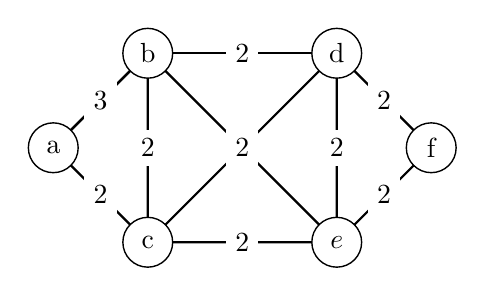
\begin{tikzpicture}[scale=1.2]
    %\SetVertexMath
    %\SetVertexNoLabel
    \GraphInit[vstyle=Normal]
        \SetUpVertex
            \Vertex[x=0,y=-1]{a}
            \Vertex[x=1,y=0]{b} 
            \Vertex[x=1,y=-2]{c}
            \Vertex[x=3,y=0]{d}
            \Vertex[Math,Lpos=270,x=3,y=-2]{e}
            \Vertex[x=4,y=-1]{f}
        %\AddVertexColor{red}{b,f}
        %\SetUpEdge[style={->,bend right,ultra thick}, color=red]
        \SetUpEdge
            \Edges[label=2,style={pos=0.5}](a,b,c,d,e,f,d,b,e,c,a)
            \Edge[label=3](a)(b)
\end{tikzpicture}

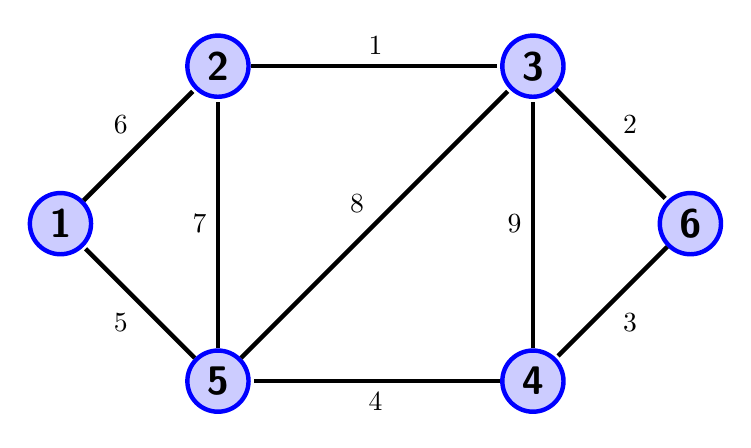
\begin{tikzpicture}[shorten >=1pt, auto, node distance=3cm, ultra thick,
   node_style/.style={circle,draw=blue,fill=blue!20!,font=\sffamily\Large\bfseries},
   edge_style/.style={draw=black, ultra thick}]

    \node[node_style] (v1) at (-2,2) {2};
    \node[node_style] (v2) at (2,2) {3};
    \node[node_style] (v3) at (4,0) {6};
    \node[node_style] (v4) at (2,-2) {4};
    \node[node_style] (v5) at (-2,-2) {5};
    \node[node_style] (v6) at (-4,0) {1};
    \draw[edge_style]  (v1) edge node{1} (v2);
    \draw[edge_style]  (v2) edge node{2} (v3);
    \draw[edge_style]  (v3) edge node{3} (v4);
    \draw[edge_style]  (v4) edge node{4} (v5);
    \draw[edge_style]  (v5) edge node{5} (v6);
    \draw[edge_style]  (v6) edge node{6} (v1);
    \draw[edge_style]  (v5) edge node{7} (v1);
    \draw[edge_style]  (v5) edge node{8} (v2);
    \draw[edge_style]  (v4) edge node{9} (v2);
    \end{tikzpicture}

% Second method
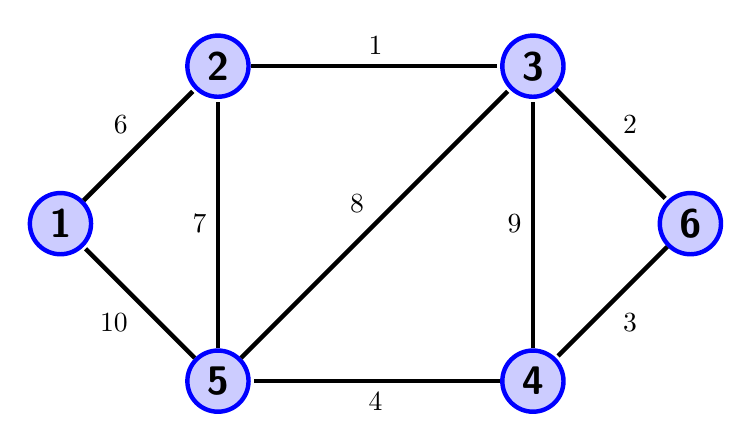
\begin{tikzpicture}[shorten >=1pt, auto, node distance=3cm, ultra thick]
   \begin{scope}[every node/.style={circle,draw=blue,fill=blue!20!,font=\sffamily\Large\bfseries}]
    \node (v1) at (-2,2) {2};
    \node (v2) at (2,2) {3};
    \node (v3) at (4,0) {6};
    \node (v4) at (2,-2) {4};
    \node (v5) at (-2,-2) {5};
    \node (v6) at (-4,0) {1};
   \end{scope}
   \begin{scope}[every edge/.style={draw=black,ultra thick}]
    \draw  (v1) edge node{1} (v2);
    \draw  (v2) edge node{2} (v3);
    \draw  (v3) edge node{3} (v4);
    \draw  (v4) edge node{4} (v5);
    \draw  (v5) edge node{10} (v6);
    \draw  (v6) edge node{6} (v1);
    \draw  (v5) edge node{7} (v1);
    \draw  (v5) edge node{8} (v2);
    \draw  (v4) edge node{9} (v2);
   \end{scope}
\end{tikzpicture}

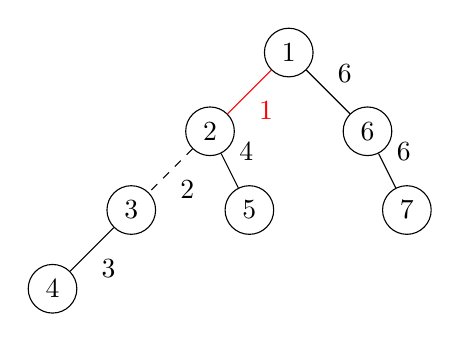
\begin{tikzpicture}[auto]
   \begin{scope}[every node/.style={circle,draw=black}]
    \node (v1) at (0,0) {1};
    \node (v2) at (-1,-1) {2};
    \node (v3) at (-2,-2) {3};
    \node (v4) at (-3,-3) {4};
    \node (v5) at (-0.5,-2) {5};
    \node (v6) at (1,-1) {6};
    \node (v7) at (1.5,-2) {7};
   \end{scope}
   \begin{scope}[every edge/.style={draw=black}]
    \draw  (v1) edge[red] node{1} (v2);
    \draw  (v2) [dashed] edge node{2} (v3);
    \draw  (v2) edge node{4} (v5);
    \draw  (v3) edge node{3} (v4);
    \draw  (v1) edge node{6} (v6);
    \draw  (v6) edge node{6} (v7);
   \end{scope}
\end{tikzpicture}


\end{document}